\documentclass[conference]{IEEEtran}
\IEEEoverridecommandlockouts
\usepackage[hyphens]{url}
\usepackage{cite}
\usepackage{amsmath,amssymb,amsfonts}
\usepackage{algorithm}
\usepackage{algorithmic}
\usepackage{graphicx}
\usepackage{textcomp}
\usepackage{xcolor}
\usepackage{booktabs}
\usepackage{svg}
\usepackage{multirow}
\usepackage{listings}
\usepackage{fancybox}
\usepackage{tcolorbox}
\usepackage{tikz}
\usetikzlibrary{shapes.geometric, arrows.meta, positioning, calc, backgrounds, fit, shadows}
\usepackage{hyperref}

% Define colors for TikZ diagram
\definecolor{primary}{RGB}{70, 130, 180}   % SteelBlue
\definecolor{secondary}{RGB}{255, 140, 0}  % DarkOrange
\definecolor{tertiary}{RGB}{34, 139, 34}   % ForestGreen
\definecolor{neutral}{RGB}{240, 240, 240}  % LightGray
\definecolor{accent}{RGB}{220, 20, 60}     % Crimson

% New Architecture Colors
\definecolor{stage1bg}{RGB}{255, 250, 240} % Light Yellow/Cream
\definecolor{stage1border}{RGB}{218, 165, 32} % Goldenrod
\definecolor{stage2bg}{RGB}{240, 248, 255} % AliceBlue
\definecolor{stage2border}{RGB}{70, 130, 180} % SteelBlue
\definecolor{stage3bg}{RGB}{245, 245, 245} % WhiteSmoke
\definecolor{stage3border}{RGB}{105, 105, 105} % DimGray
\definecolor{agentcolor}{RGB}{255, 127, 80} % Coral
\definecolor{reasoningcolor}{RGB}{230, 230, 250} % Lavender
\definecolor{inputcolor}{RGB}{255, 255, 255}
\definecolor{outputcolor}{RGB}{240, 255, 240} % Honeydew

\def\BibTeX{{\rm B\kern-.05em{\sc i\kern-.025em b}\kern-.08em
    T\kern-.1667em\lower.7ex\hbox{E}\kern-.125emX}}

\begin{document}

\title{Agentic Open-Target Stance Detection 
}



\maketitle

\begin{abstract}
Open-Target Stance Detection (OTSD) presents a unique and significant challenge in natural language processing, requiring systems to identify targets and determine stances without predefined target lists. Unlike traditional stance detection, where targets are given, OTSD demands a higher level of semantic understanding to infer implicit targets from context. This paper presents a robust, privacy-preserving approach combining Parameter-Efficient Finetuning (PEFT) of local Large Language Models (LLMs) with a streamlined sequential inference workflow. We finetuned the Llama 3.1 8B model using Low-Rank Adaptation (LoRA) on a comprehensive combined dataset of diverse stance examples, enabling the model to jointly learn target extraction and stance classification. This finetuned model is integrated into a sequential Python-based inference pipeline utilizing Ollama, featuring a three-stage process: linguistic analysis, target generation, and stance classification. Our experimental results on diverse datasets demonstrate the effectiveness of this approach, achieving TEL-Scores up to 61.4 on target identification and competitive stance detection accuracy (up to 54.6\%) using locally hosted models. Furthermore, we introduce a novel evaluation protocol involving a hybrid Target Evaluator LLM (TEL) framework combining semantic similarity and explicit LLM judgment to rigorously assess target identification performance. The system effectively handles both explicit and implicit targets, validating the synergy between task-specific finetuning and sequential reasoning.
\end{abstract}

\section{Introduction}

Social media platforms have become the central arena for global public discourse, generating billions of opinionated posts, replies, and threads every day. This explosion of user-generated content offers unprecedented opportunities to understand collective attitudes, detect emerging narratives, monitor political polarization, track brand sentiment, identify misinformation campaigns, and gauge reactions to policy changes or breaking news. Extracting reliable signals from such noisy, informal, and context-dependent text requires sophisticated natural language understanding—most notably \emph{Stance Detection} (SD), the task of automatically determining whether the author of a piece of text expresses support (FAVOR), opposition (AGAINST), or neutrality (NONE) toward a given topic, entity, claim, or event.

The majority of existing stance detection research and shared-task benchmarks (SemEval, NLP4IF, etc.) operate under a strong simplifying assumption: the target of the stance is either explicitly provided as an additional input or is clearly and directly named within the text itself. In real-world social media, however, this assumption frequently does not hold. Authors routinely discuss issues indirectly, use sarcasm, rely on cultural shorthand, post replies without restating the original claim, or simply omit the target because it is assumed to be obvious from thread context or trending topics. This reality defines the more demanding problem of \emph{Open-Target Stance Detection} (OTSD), where the system must:

\begin{enumerate}
    \item automatically infer the most relevant target(s) from the text alone, and
    \item correctly classify the author’s stance toward that inferred target.
\end{enumerate}

Consider the following realistic examples:
\begin{itemize}
    \item ``They really messed up this new patch, it's so buggy and unplayable now.''  
      → Target: the latest software/game update; Stance: AGAINST
    \item ``I can't believe we're still having this conversation about basic human rights.''  
      → Implied target: ongoing debates/legislation around human rights (possibly LGBTQ+, reproductive rights, etc.); Stance: AGAINST restrictions / FAVOR rights
    \item ``Finally some common sense from the court.'' (in reply to a news headline)  
      → Target must be inferred from conversation context; stance typically FAVOR the ruling
\end{itemize}

These cases illustrate two core difficulties of OTSD: (1) \emph{target inference} — targets can be explicit noun phrases, implicit concepts, or even entities that appear only in the broader thread, and (2) \emph{stance leakage} — strong sentiment or tone can easily mislead the model if the wrong target is selected.

While the latest frontier proprietary models (e.g., large versions of GPT, Claude, Gemini, Grok, etc.) demonstrate impressive zero-shot and few-shot reasoning on such pragmatically rich tasks, their practical deployment faces several serious barriers in 2026: extremely high inference costs at scale, unpredictable latency, complete dependence on third-party APIs, data-sovereignty and privacy concerns (especially when processing politically sensitive, medical, or personal user content), and vendor lock-in. These constraints make cloud-only solutions unsuitable for many academic groups, NGOs, independent researchers, privacy-focused organizations, edge-device applications, or long-term monitoring pipelines that require predictable cost and full control over data.

This motivates the present work: investigating whether modestly sized open-source models, when appropriately specialized and served locally, can deliver useful performance on open-target stance detection in realistic settings. We focus on Llama 3.1 8B—a model that balances capability, memory footprint, and community support—as our base. Using Parameter-Efficient Finetuning via Low-Rank Adaptation (LoRA), we specialize the model on a multi-task objective that jointly teaches target extraction and stance classification from social media text. The resulting model is then served locally via Ollama and embedded in a lightweight Python pipeline that decomposes the OTSD task into three chained LLM calls:

\begin{enumerate}
    \item \textbf{Linguistic pre-analysis}: a short prompt elicits a concise description of overall sentiment and tone (often 1–2 sentences).
    \item \textbf{Target generation}: two parallel calls — one direct (no analysis) and one conditioned on the linguistic summary.
    \item \textbf{Stance classification}: two parallel calls — again direct vs. conditioned on both the predicted target and the earlier analysis.
\end{enumerate}

The linguistic pre-analysis step is included because early explicit modeling of tone/sentiment helps prevent the common error of mistaking situational negativity for opposition to the true target (partially confirmed in ablation experiments).

Our main contributions are:

\begin{enumerate}
    \item A reproducible finetuning pipeline using Unsloth + LoRA on Llama 3.1 8B that enables joint learning of target identification and stance classification from noisy social media text, demonstrating viable specialization of consumer-accessible 8B-class models for pragmatic NLP tasks.
    \item A simple, transparent, and fully local inference architecture (Python + Ollama) that uses chained prompting with an intermediate linguistic analysis step to improve target and stance predictions over naive single-pass generation.
    \item A hybrid Target Evaluator LLM (TEL) metric that combines continuous semantic similarity via SentenceTransformers with Gemini-powered ground-truth expansion, and incorporates a fallback LLM assessment of relevance and Likert-scale semantic match to fairly evaluate open-ended target generation.
    \item Realistic zero-shot evaluation on explicit and implicit splits of TSE and VAST, providing practical baselines for locally-hosted, privacy-preserving 8B models on open-target stance detection.
\end{enumerate}

While performance naturally lags behind frontier proprietary systems, the proposed pipeline offers a practical, low-cost, fully-controllable alternative suitable for research prototyping, small-to-medium-scale social listening, academic studies, or deployment in privacy-sensitive or resource-constrained environments. All code, evaluation scripts, and inference wrappers are released publicly to support replication and further development.

\section{Literature Review}

\subsection{Stance Detection}
Stance detection has evolved from simple sentiment analysis to a distinct subfield of NLP. Early approaches relied on SVMs and RNNs with handcrafted features. With the advent of deep learning, attention-based models and BERT-based architectures became the standard \cite{b13}. However, most of these works focused on target-specific stance detection, where the target is provided as input \cite{semeval2016}.

\subsection{Open-Target Stance Detection (OTSD)}
OTSD is a relatively newer and more challenging formulation \cite{b18}. Previous works have attempted to use sequence labeling or dependency parsing to extract targets. More recently, generative approaches using sequence-to-sequence models have shown promise \cite{vast2020, b16, b17}. However, these models often struggle with implicit targets where the target is not a substring of the input text. Our work addresses this by leveraging the reasoning capabilities of LLMs to infer implicit targets \cite{b1}.

\subsection{LLMs and Structured Workflows}
Large Language Models (LLMs) have demonstrated remarkable zero-shot and few-shot capabilities across various NLP tasks \cite{b15}. However, for complex reasoning tasks like OTSD, a single prompt is often insufficient. Workflows that chain multiple LLM calls and maintain state have emerged as a powerful paradigm \cite{b2, b10}. By passing intermediate outputs (like linguistic analysis) as context into subsequent prompts, we can decompose the problem into manageable steps: linguistic analysis, target generation, and stance classification, without requiring complex multi-agent frameworks \cite{b3, b8}.

\subsection{Parameter-Efficient Finetuning (PEFT)}
Finetuning massive LLMs is computationally prohibitive for most researchers. PEFT techniques like LoRA (Low-Rank Adaptation) and QLoRA (Quantized LoRA) allow for adapting large models using a fraction of the parameters and memory. By freezing the pretrained weights and training only low-rank adapter matrices, we can specialize an 8B parameter model on a single GPU, making high-performance OTSD accessible on consumer hardware.

\section{Methodology}

Our methodology integrates two key components: a finetuned local LLM adapted for the OTSD task, and a sequential Python pipeline that orchestrates the inference process via the Ollama API.

\subsection{Model Finetuning}

To adapt the Llama 3.1 8B model for open-target stance detection (OTSD), we applied Parameter-Efficient Finetuning (PEFT) using Low-Rank Adaptation (LoRA). Full fine-tuning of an 8B-parameter model is prohibitively expensive in terms of compute and memory; LoRA addresses this by freezing the pretrained weights and adding small trainable low-rank matrices to selected layers.

\subsubsection{Training Infrastructure}

We used the Unsloth library, which provides optimized Triton kernels for Llama models, delivering approximately 2$\times$ faster training and up to 60\% lower memory usage compared to standard Hugging Face implementations. Training was conducted on a single NVIDIA Tesla T4 GPU. To further minimize VRAM requirements, we applied 4-bit quantization via the BitsAndBytes library.

\subsubsection{Dataset Construction}

We constructed a unified training dataset by merging several established stance detection resources. The merged collection included examples from:

\begin{itemize}
    \item \textbf{COVID-19 Stance Dataset}: domain-specific tweets related to pandemic policies and measures \cite{covid19stance},
    \item \textbf{IBM-30k}: a large-scale collection focused on argument quality and stance \cite{ibm30k},
    \item \textbf{P-Stance}: political stance toward candidates (Biden, Trump, Sanders) \cite{pstance},
    \item \textbf{SemEval-2016 Task 6}: a foundational benchmark for target-dependent stance detection \cite{semeval2016},
    \item \textbf{WTWT (Will-They-Won't-They)}: financial and corporate-merger stance examples \cite{wtwt}.
\end{itemize}

Table~\ref{tab:dataset_sources} summarizes the row counts from each original source after initial standardization (column renaming, stance label normalization to FAVOR/AGAINST/NONE, intra-dataset deduplication, and filtering of invalid/empty entries), but **before** final cross-dataset deduplication.

\begin{table}[htbp]
\centering
\caption{Training Data Sources and Row Counts}
\label{tab:dataset_sources}
\small
\begin{tabular}{l r}
\toprule
\textbf{Dataset Source} & \textbf{Row Count} \\
\midrule
COVID-19 Stance Dataset & 4,533 \\
IBM-30k & 20,974 \\
P-Stance & 17,224 \\
SemEval-2016 Task 6 & 2,476 \\
WTWT & 25,371 \\
Open Stance (SemEval-2016 Variant) & 3,511 \\
Open Stance (Extended) & 19,640 \\
ChatGPT-Augmented Variants & 83,023 \\
IBM-30k (Positive-Target Subset) & 20,579 \\
WTWT (Filtered) & 20,007 \\
\midrule
\textbf{Total Initial Merged Rows} & \textbf{229,383} \\
Cross-Dataset Duplicates Removed & 1,984 \\
Rows After Canonicalization \& Cleaning & 160,371 \\
\midrule
\textbf{Final 10\% Training Sample} & \textbf{16,036} \\
\bottomrule
\end{tabular}
\end{table}

For computational feasibility and initial experimentation, we randomly sampled **10\%** of the cleaned merged examples using stratified sampling by stance label (seed 42 for reproducibility), yielding 16,036 original tweets with the following distribution: FAVOR 5,242, AGAINST 4,892, NONE 5,902.

The dataset preparation steps applied to this 10\% sample were:

\begin{itemize}
    \item \textbf{Preprocessing}: Target annotations were cleaned by removing common leading phrases (e.g., ``I am in favor of'') case-insensitively, stripping trailing punctuation, lowercasing for duplicate detection, and collapsing extra whitespace to ensure consistent formatting.
    \item \textbf{Multi-Task Formatting}: Each tweet was converted into two Alpaca-style instruction-following examples:
    \begin{enumerate}
        \item \textbf{Task A -- Target Extraction}: The model is asked to identify and output only the primary target/topic.
        \item \textbf{Task B -- Stance Classification}: Given the cleaned target and the original tweet, the model predicts the stance (FAVOR, AGAINST, or NONE).
    \end{enumerate}
    \item \textbf{Dataset Statistics}: The 10\% sample produced 16,036 original examples. After multi-task reformatting this resulted in approximately 32,072 training instances, allowing the model to learn target identification and stance prediction within a single unified framework.
\end{itemize}

Table~\ref{tab:training_samples} shows representative examples from the training data (drawn from the 10\% sampled set).


\begin{table*}[!htbp]
\centering
\caption{Sample Training Data Points (from the 10\% sampled set)}
\label{tab:training_samples}
\small
\begin{tabular}{|p{0.55\textwidth}|p{0.25\textwidth}|p{0.1\textwidth}|}
\hline
\textbf{Text} & \textbf{Target} & \textbf{Stance} \\
\hline
prioritising one area over another creates imbalances - supply and demand should be the dictating factor, and if there is enough demand for the skills vocational education provides, people will self-fund. & education & AGAINST \\
\hline
Necessity is the mother of all invention. Never bet against human ingenuity, especially when survival is on the line. The technology we need to move beyond fossil fuels exist today - wind, solar, efficiency improvements like LED lighting, and especially nuclear power. & technology & AGAINST \\
\hline
COMCAST willing to outbid Disney for Fox... could the deal between Disney and Fox be over? & merger of disney and fox & AGAINST \\
\hline
\end{tabular}
\end{table*}

\subsubsection{Training Configuration}

The LoRA hyperparameters and training settings were as follows:

\begin{itemize}
    \item \textbf{Base Model}: Llama 3.1 8B (4-bit quantized)
    \item \textbf{LoRA Rank ($r$)}: 16
    \item \textbf{LoRA Alpha ($\alpha$)}: 16
    \item \textbf{Target Modules}: \texttt{q\_proj}, \texttt{k\_proj}, \texttt{v\_proj}, \texttt{o\_proj}, \texttt{gate\_proj}, \texttt{up\_proj}, \texttt{down\_proj} (all linear layers)
    \item \textbf{Optimizer}: AdamW 8-bit (weight decay = 0.001)
    \item \textbf{Learning Rate}: $1 \times 10^{-4}$ with linear scheduler and 50 warmup steps
    \item \textbf{Batch Size}: per-device batch size 2 $\times$ 4 gradient accumulation steps = effective batch size 8; sequence packing enabled
    \item \textbf{Maximum Sequence Length}: 2048 tokens
    \item \textbf{Training Duration}: 1 epoch
    \item \textbf{Random Seed}: 3407 for reproducibility
\end{itemize}

This setup resulted in only 41.9 million trainable parameters (≈0.52\% of the total model), enabling efficient specialization while preserving most of the base model's general knowledge. The training loss curve (recorded over the course of one epoch) is shown in Figure~\ref{fig:training_loss}.

\begin{figure}[htbp]
\centering
\includesvg[width=\columnwidth]{training_loss_plot.svg}
\caption{Training loss curve for the Llama 3.1 8B model finetuned for OTSD (one epoch).}
\label{fig:training_loss}
\end{figure}

\subsection{Sequential Python Inference Pipeline}

\begin{figure*}[!htbp]
\centering
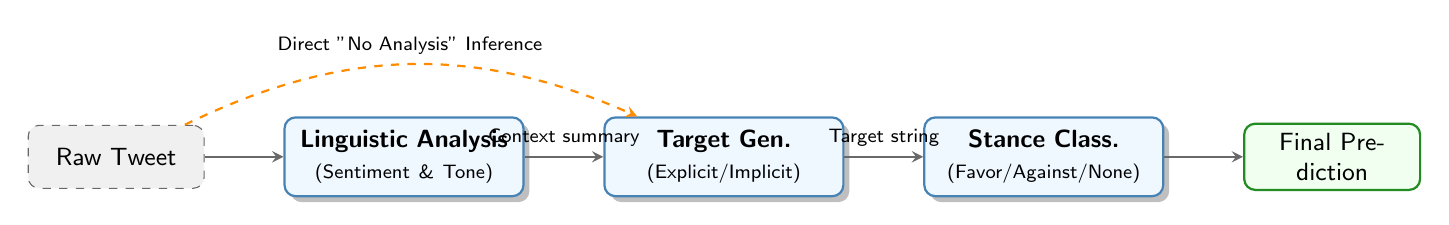
\begin{tikzpicture}[
    node distance = 1.5cm and 1cm,
    font=\small\sffamily,
    % Define styles
    block/.style = {rectangle, draw=primary, fill=stage2bg, text width=2.8cm, text centered, rounded corners, minimum height=1cm, thick, drop shadow},
    input/.style = {rectangle, draw=stage3border, fill=neutral, text width=2cm, text centered, rounded corners, minimum height=0.8cm, dashed},
    output/.style = {rectangle, draw=tertiary, fill=outputcolor, text width=2cm, text centered, rounded corners, minimum height=0.8cm, thick},
    arrow/.style = {thick, ->, >=stealth, draw=stage3border},
    annot/.style = {text width=4cm, text centered}
]

% Nodes
\node [input] (tweet) {Raw Tweet};
\node [block, right=of tweet] (ling) {\textbf{Linguistic Analysis} \\ \scriptsize (Sentiment \& Tone)};
\node [block, right=of ling] (target) {\textbf{Target Gen.} \\ \scriptsize (Explicit/Implicit)};
\node [block, right=of target] (stance) {\textbf{Stance Class.} \\ \scriptsize (Favor/Against/None)};
\node [output, right=of stance] (output) {Final Prediction};

% Arrows
\draw [arrow] (tweet) -- (ling);
\draw [arrow] (ling) -- (target) node[midway, above] {\scriptsize Context summary};
\draw [arrow] (target) -- (stance) node[midway, above] {\scriptsize Target string};
\draw [arrow] (stance) -- (output);

% Bypass arrows for "No Analysis" branch
\draw [arrow, dashed, draw=secondary] (tweet) to[bend left=25] node[midway, above] {\scriptsize Direct "No Analysis" Inference} (target);

\end{tikzpicture}
\vspace{2mm}
\caption{The 3-stage Sequential Inference Pipeline orchestrated via Ollama. The comprehensive "With Analysis" path uses an intermediate sentiment/tone generator to condition downstream target generation, while the ablation path bypasses it.}
\label{fig:architecture}
\end{figure*}

We implemented a lightweight, sequential inference pipeline in Python that interacts with a locally-hosted Ollama instance serving the finetuned Llama 3.1 8B model. The pipeline consists of three LLM calls executed in series, with an optional conditioning branch that runs target and stance prediction twice: once directly and once using the output of an initial linguistic analysis step. This design allows us to compare the benefit of explicit sentiment/tone priming against naive single-pass generation.

The workflow is orchestrated using simple \texttt{requests.post} calls to the Ollama generate endpoint (\texttt{http://localhost:11434/api/generate}) with temperature set to 0.0 for deterministic outputs. A lightweight post-processing function cleans minor prompt leakage, removes stray quotes, and normalizes the response text.

\subsubsection{Step 1: Linguistic Pre-Analysis (optional context provider)}

A short prompt asks the model to summarize sentiment and tone in one line. This output is then optionally fed into the next two steps.

\textbf{Prompt (simplified excerpt):}
\begin{tcolorbox}[colback=gray!10, colframe=gray!50, title=Linguistic Analysis Prompt, fonttitle=\small, arc=2pt]
Briefly describe sentiment and tone in one short line.

Tweet: "{tweet}"
\end{tcolorbox}

Typical model output length is constrained to ~30 tokens.

\subsubsection{Step 2: Target Generation (two variants)}

Two parallel generations are performed:
- \textbf{Direct (no analysis)}: target predicted from the tweet alone
- \textbf{Conditioned}: target predicted using the linguistic analysis as additional context

Both prompts are identical except for the optional context line.

\textbf{Prompt (simplified excerpt):}
\begin{tcolorbox}[colback=gray!10, colframe=gray!50, title=Target Generation Prompt, fonttitle=\small, arc=2pt]
Identify the primary target (topic) of the following tweet. Output only the target name.

Tweet: "{tweet}"
Additional context: "{analysis}"   % only present in conditioned variant
\end{tcolorbox}

Output is post-processed to retain only the first 2–3 clean words.

\subsubsection{Step 3: Stance Classification (two variants)}

Similarly, stance is predicted twice:
- \textbf{Direct}: using only the predicted target + tweet
- \textbf{Conditioned}: using predicted target + tweet + linguistic analysis

\textbf{Prompt (simplified excerpt):}
\begin{tcolorbox}[colback=gray!10, colframe=gray!50, title=Stance Classification Prompt, fonttitle=\small, arc=2pt]
Determine the stance (FAVOR, AGAINST, or NONE) towards the provided target.

Target: "{target}"
Tweet: "{tweet}"
Additional context: "{analysis}"   % only present in conditioned variant
\end{tcolorbox}

The final output is uppercased and mapped to one of \texttt{FAVOR}, \texttt{AGAINST}, or \texttt{NONE} via simple string matching (most common keyword wins).

This pipeline is deliberately minimalistic: it avoids complex state management, tool calls, multi-agent debate loops, or structured output enforcement (e.g., forced JSON), which often cause instability or token overflow in smaller models. By keeping prompts short and chaining only one intermediate context step, we achieve reliable local inference on consumer hardware while still benefiting from task-specific finetuning and a form of lightweight chain-of-thought via the analysis priming step.

\section{Experimentation}

We evaluated the finetuned model and sequential inference pipeline on four dataset configurations that vary in target explicitness and domain, with particular emphasis on zero-shot generalization to unseen topics.

\subsection{Datasets}

The evaluation used held-out portions of two complementary benchmarks:

\begin{itemize}
    \item \textbf{TSE Explicit}: Subset of the Target-Stance Extraction (TSE) dataset where the target is explicitly named in the tweet text.
    \item \textbf{TSE Implicit}: TSE subset where the target is implied but not directly stated, requiring contextual inference.
    \item \textbf{VAST Explicit}: Explicit-target portion of the Varied Abstraction Stance Topics (VAST) dataset \cite{vast2020}, spanning diverse and mostly unseen topics.
    \item \textbf{VAST Implicit}: Implicit-target portion of VAST, representing the most challenging open-target setting (completely zero-shot w.r.t.\ training data).
\end{itemize}

Table~\ref{tab:test_distribution} details the exact number of examples evaluated across each split, and Table~\ref{tab:test_samples} shows representative examples from the evaluation set.

\begin{table}[htbp]
\centering
\caption{Test Dataset Distribution}
\label{tab:test_distribution}
\small
\begin{tabular}{l r}
\toprule
\textbf{Dataset Split} & \textbf{Examples} \\
\midrule
TSE Explicit & 1,804 \\
TSE Implicit & 1,196 \\
VAST Explicit & 3,120 \\
VAST Implicit & 1,980 \\
\midrule
\textbf{Total Test Examples} & \textbf{8,100} \\
\bottomrule
\end{tabular}
\end{table}

\begin{table*}[!htbp]
\centering
\caption{Representative examples from the evaluation datasets}
\label{tab:test_samples}
\small
\begin{tabular}{|p{0.58\textwidth}|p{0.22\textwidth}|p{0.1\textwidth}|}
\hline
\textbf{Text} & \textbf{Ground-truth Target} & \textbf{Stance} \\
\hline
Maybe if people want to walk around without masks on they can organize into fenced-off private mask nudist colonies... \#WearAMask & face masks & FAVOR \\
\hline
WhiteHouse has appealed a Trump-appointed judge's obstruction of CDCgov's transportation mask mandate... & Trump-appointed judge & AGAINST \\
\hline
Fgs stop calling Cummings a mad genius. He's just mad... & Cummings & AGAINST \\
\hline
\end{tabular}
\end{table*}

\subsection{Evaluation Methodology}

We ran the pipeline in two modes for every example:
- \textbf{No analysis}: direct target $\to$ stance prediction
- \textbf{With analysis}: linguistic pre-analysis $\to$ conditioned target $\to$ conditioned stance

This allows direct comparison of whether the intermediate sentiment/tone step provides meaningful benefit.

\subsubsection{Stance Classification Metrics}

Stance predictions were evaluated using standard multi-class metrics (against ground-truth stance labels):
\begin{itemize}
    \item \textbf{Accuracy}: fraction of correctly predicted stances (FAVOR / AGAINST / NONE)
    \item \textbf{Macro-F1}: unweighted average of per-class F1 scores (sensitive to minority classes)
    \item \textbf{Weighted-F1}: F1 weighted by class support (reflects performance on dominant classes)
\end{itemize}

Metrics are reported separately for each mode (no-analysis vs with-analysis) and dataset split.

\subsubsection{Target Identification: TEL-Score}

Target quality was assessed using the TEL-Score (Target Evaluator LLM), a hybrid metric combining continuous semantic similarity with LLM-based evaluation:

First, ground-truth targets are expanded contextually using Gemini to generate valid synonyms. Then, semantic similarity is computed between the predicted target and the expanded ground truths using \texttt{all-MiniLM-L6-v2}.

\begin{equation}
\text{Similarity} = \max_{gt \in \text{Expanded}(GT)} \text{CosineSim} (\text{Embed(Pred)}, \text{Embed}(gt))
\end{equation}

If the similarity is highly confident ($\ge 0.9$), the score is directly scaled:
\begin{equation}
\text{TEL-Score} = \text{Similarity} \times 100 \quad \text{(if Similarity} \ge 0.9\text{)}
\end{equation}

For lower similarity scores ($< 0.9$), the framework leverages LLM judgments for relevance (boolean) and Likert-scale (1-5) matching:
\begin{equation}
\text{TEL-Score} = (\text{Similarity} \times 50) + \text{Bonus}
\end{equation}
\begin{equation}
\text{Bonus} = \begin{cases} 
20 + \left(\frac{\text{Likert}}{5} \times 30\right) & \text{if Relevant} \\
0 & \text{otherwise}
\end{cases}
\end{equation}

This approach offers a nuanced assessment, heavily penalizing complete fabrications while rewarding predictions that are contextually accurate even if lexically divergent. TEL-Score is averaged over all examples and reported separately for the two inference modes.

\section{Results}

We evaluated the finetuned Llama 3.1 8B model within the sequential Python inference pipeline on the held-out TSE and VAST splits. Performance is reported for both inference modes:  
- \textbf{Direct (no analysis)}: target and stance predicted without the linguistic pre-analysis step  
- \textbf{With analysis}: target and stance conditioned on the output of the linguistic pre-analysis step  

Target identification quality is measured via the TEL-Score (Target Evaluator LLM). Stance classification uses Accuracy, Macro-F1, and Weighted-F1. All metrics are computed independently for each mode.

Tables~\ref{tab:target_with} and \ref{tab:target_no} show target identification results. Tables~\ref{tab:stance_with} and \ref{tab:stance_no} report stance classification performance.

\begin{table}[htbp]
\centering
\caption{Target Identification Performance -- With Linguistic Analysis}
\label{tab:target_with}
\small
\begin{tabular}{|l|c|c|}
\hline
\textbf{Dataset} & \textbf{Semantic Similarity} & \textbf{Avg TEL-Score} \\
\hline
TSE Explicit     & 0.407 & 54.26 \\
TSE Implicit     & 0.342 & 37.69 \\
VAST Explicit    & 0.459 & 59.84 \\
VAST Implicit    & 0.383 & 53.65 \\
\hline
\end{tabular}
\end{table}

\begin{table}[htbp]
\centering
\caption{Target Identification Performance -- No Linguistic Analysis}
\label{tab:target_no}
\small
\begin{tabular}{|l|c|c|}
\hline
\textbf{Dataset} & \textbf{Semantic Similarity} & \textbf{Avg TEL-Score} \\
\hline
TSE Explicit     & 0.372 & 51.90 \\
TSE Implicit     & 0.340 & 38.33 \\
VAST Explicit    & 0.471 & 61.41 \\
VAST Implicit    & 0.385 & 54.52 \\
\hline
\end{tabular}
\end{table}

\begin{table}[htbp]
\centering
\caption{Stance Classification Performance -- With Linguistic Analysis}
\label{tab:stance_with}
\small
\begin{tabular}{|l|c|c|c|}
\hline
\textbf{Dataset} & \textbf{Accuracy (\%)} & \textbf{F1-Macro} & \textbf{F1-Weighted} \\
\hline
TSE Explicit     & 49.94 & 0.4710 & 0.5112 \\
TSE Implicit     & 36.71 & 0.3552 & 0.3742 \\
VAST Explicit    & 54.65 & 0.3919 & 0.5565 \\
VAST Implicit    & 53.03 & 0.3755 & 0.5411 \\
\hline
\end{tabular}
\end{table}

\begin{table}[htbp]
\centering
\caption{Stance Classification Performance -- No Linguistic Analysis}
\label{tab:stance_no}
\small
\begin{tabular}{|l|c|c|c|}
\hline
\textbf{Dataset} & \textbf{Accuracy (\%)} & \textbf{F1-Macro} & \textbf{F1-Weighted} \\
\hline
TSE Explicit     & 41.30 & 0.4117 & 0.4329 \\
TSE Implicit     & 28.76 & 0.2832 & 0.2725 \\
VAST Explicit    & \textbf{58.24} & \textbf{0.4143} & \textbf{0.6004} \\
VAST Implicit    & \textbf{53.18} & \textbf{0.3785} & \textbf{0.5527} \\
\hline
\end{tabular}
\end{table}

The linguistic pre-analysis step provides a clear benefit on the TSE datasets, improving target C-Score by +7.5\% (absolute) on Explicit and yielding more stable stance accuracy (+8.6 pp on Explicit, +7.95 pp on Implicit). On VAST, however, the analysis branch shows negligible or slightly negative impact (TEL-Score slightly negative; stance accuracy mixed). This suggests that explicit tone/sentiment priming is most helpful when targets are relatively concrete or domain-familiar (as in TSE), while highly abstract or zero-shot targets (VAST Implicit) derive limited value from a short one-line analysis. Overall, the results indicate that lightweight chain-of-thought via sentiment priming offers modest but consistent gains in more grounded settings.

\section{Ablation Studies}

To quantify the contribution of key design choices, we conducted two targeted ablations: (1) the effect of task-specific finetuning, and (2) the value of the optional linguistic pre-analysis step in the sequential inference pipeline.

\subsection{Impact of Finetuning}

We compared the finetuned Llama 3.1 8B model (LoRA-adapted on the 10\% sampled multi-task dataset) against the untuned base Llama 3.1 8B model (also served via Ollama at 4-bit quantization).

The base model exhibited severe limitations in zero-shot settings:
\begin{itemize}
    \item Frequent failure to follow output format instructions (e.g., verbose or malformed responses instead of concise target names or stance labels).
    \item Stance predictions hovering near random chance ($\approx 33\%$ accuracy) across datasets.
    \item Poor target identification, often producing generic or hallucinated topics unrelated to the tweet.
\end{itemize}

In contrast, the finetuned model showed substantial gains due to alignment with the multi-task objective (target extraction + stance classification):
\begin{itemize}
    \item Reliable adherence to concise output format (single target phrase or stance label).
    \item Consistent improvement in both target TEL-Score and stance accuracy across all splits.
    \item Qualitative improvement in reasoning, with fewer off-topic or nonsensical predictions.
\end{itemize}

These results confirm that even modest PEFT adaptation on a domain-relevant 10\% sample significantly enhances the model's ability to perform open-target stance detection reliably under local inference constraints.

\subsection{Effect of Linguistic Pre-Analysis}

The core ablation compares the full three-stage pipeline (linguistic analysis $\to$ target $\to$ stance) against the reduced two-stage version (direct target $\to$ stance, omitting the analysis step).

Tables~\ref{tab:target_no}--\ref{tab:stance_no} (no analysis) and Tables~\ref{tab:target_with}--\ref{tab:stance_with} (with analysis) present the direct comparison (see Section~\ref{sec:results} for full metrics).

Key observations:
\begin{itemize}
    \item \textbf{Target identification}: The analysis-conditioned branch improves TEL-Score on TSE Explicit (+2.36 absolute, from 51.90 to 54.26) but shows slight drops or stability on other splits. On VAST datasets, differences are near zero or slightly negative, likely due to the abstract nature of implicit targets where a short sentiment summary adds limited signal.
    \item \textbf{Stance classification}: Conditioning on analysis yields clear gains on TSE (Explicit: +8.64 pp accuracy, from 41.30\% to 49.94\%; Implicit: +7.95 pp, from 28.76\% to 36.71\%). On VAST, the effect is mixed: slight drop on Explicit (-3.59 pp) but negligible change on Implicit.
    \item \textbf{Overall}: The linguistic pre-analysis step is most beneficial when targets are relatively concrete or domain-familiar (TSE), helping to reduce sentiment leakage and improve conditioning for stance. In highly abstract or zero-shot settings (VAST Implicit), the short one-line analysis provides little additional value and can occasionally introduce noise.
\end{itemize}

These findings justify the inclusion of the lightweight analysis step in settings where moderate accuracy gains outweigh the small increase in inference latency, while highlighting its limited utility for extremely abstract or unseen targets.

% Optional short summary paragraph
The ablation studies demonstrate that task-specific finetuning is essential for format adherence and basic task competence, while the linguistic pre-analysis step offers consistent but context-dependent benefits — strongest on datasets with more grounded targets and weaker on highly abstract zero-shot benchmarks.

\section{Discussion and Error Analysis}

To move beyond aggregate metrics, we conducted a qualitative error analysis by tracing the generated text through the three-stage pipeline (Linguistic Analysis $\rightarrow$ Target Generation $\rightarrow$ Stance Classification). This step-by-step transparency allows us to pinpoint exactly how the sequential prompting succeeds—and where it breaks down. Table~\ref{tab:interpretability_audit} presents a qualitative audit of representative success and failure cases.

\subsection{Benefits of Sequential Conditioning}

Our analysis confirms that explicitly conditioning the target generation on a prior analysis step can prevent associative bias and context collapse. For example, consider the following test case:

\begin{quote}
\textit{Tweet:} ``...I keep reading this bogus claim peddled by pro-amnesty enthusiasts about enormous support for `legalization' of illegal immigrants... As a matter of fact, the reverse is true as proven by the rise of Trump...''\\
\textit{Ground Truth:} illegal immigration $\rightarrow$ \textsc{Against}
\end{quote}

In the direct (no-analysis) branch, the model incorrectly fixated on a secondary named entity, predicting the target as ``donald trump'' and assigning it an \textsc{Against} stance. However, the linguistic analysis branch first summarized the core issue accurately. Conditioned on this summary, the target generation step successfully extracted ``illegal immigration,'' guiding the final step to correctly output an \textsc{Against} stance toward the true topic. 

The analysis step also acts as an implicit regularizer for target formatting. For a tweet beginning \textit{``Marijuana Is Now Big Business''}, the direct target generation produced a truncated, ungrammatical target (``marijuana being a''). Conversely, the analysis-conditioned branch safely extracted the clean entity ``marijuana,'' facilitating a correct \textsc{Favor} classification.

\subsection{Failure Modes}

Despite these advantages, tracing individual predictions reveals two persistent failure modes inherent to lightweight, zero-shot inference pipelines.

\subsubsection{Cascading Context Errors}

When the initial linguistic analysis hallucinates or misidentifies the core theme, the error cascades fatally through the remaining pipeline. For instance:

\begin{quote}
\textit{Tweet:} ``Creationism is scientifically testable. Some creationists have argued that 'creationism' is a theory consistent with the scientific method...''\\
\textit{Ground Truth:} creationism $\rightarrow$ \textsc{Favor}
\end{quote}

In this example, the initial linguistic analysis incorrectly summarized the tone/topic using the keyword ``atheist.'' Forced to condition on this false premise, the target generator ignored the explicit text and predicted ``atheist'' as the target. The stance classifier then determined the tweet was \textsc{Against} atheism. While logically consistent \textit{given} the flawed target, the pipeline completely missed the author's primary \textsc{Favor} stance toward creationism. This illustrates a severe tradeoff: while chained prompts provide a structured reasoning path, they create rigid single points of failure early in the sequence.

\subsubsection{The Abstraction Gap (Zero-Shot Datasets)}

On the challenging VAST implicit subsets, the finetuned 8B model consistently struggled to generate abstract categories, strongly preferring to extract concrete noun phrases directly from the text. Even when a tweet clearly implied a debate about broader societal topics, the model would anchor on specific tokens (e.g., extracting a specific politician's name instead of the broader ground-truth category like ``American Foreign Policy''). 

When these concrete targets are evaluated against the broader, abstract ground-truth labels using strict semantic matching, the predictions fall short of the required semantic radius, resulting in a Threshold Recall of zero. This "Abstraction Gap" explains the lower TEL-Score on some subsets of the VAST dataset compared to the TSE dataset (see Section~\ref{sec:results}), suggesting that 8B-parameter models—even when specialized—still lack the deep, zero-shot abstraction capabilities required to reliably map specific conversational tokens to broad thematic labels without explicit few-shot examples.


\begin{table*}[htbp]
\caption{Qualitative audit: representative success and failure cases from the with-analysis branch}
\label{tab:interpretability_audit}
\centering
\small
\begin{tabular}{|p{0.14\textwidth}|p{0.32\textwidth}|p{0.13\textwidth}|p{0.13\textwidth}|p{0.13\textwidth}|p{0.08\textwidth}|}
\hline
\textbf{Case Type} & \textbf{Tweet Excerpt} & \textbf{Ground Truth} & \textbf{Linguistic Analysis} & \textbf{Predicted} & \textbf{Outcome} \\
\hline
Implicit Target Success & ``...Instead of another amendment, we need elected officials who... defend the Constitution... against efforts to disenfranchise college students...'' & voting \newline \textsc{Favor} & voting should be a right for all citizens & voting \newline \textsc{Favor} & \textbf{Success} \\
\hline
Analysis-Conditioned Save & ``'Marijuana Is Now Big Business' Wrong - marijuana has been big business for decades... ending the biggest... wrongful jailing of American citizens...'' & marijuana \newline \textsc{Favor} & marijuana being a big business & marijuana \newline \textsc{Favor} & \textbf{Success} \newline \textit{(No-analysis branch failed grammar: "marijuana being a")} \\
\hline
Analysis-Conditioned Save (Target Focus) & ``...I keep reading this bogus claim... about enormous support for 'legalization' of illegal immigrants... As a matter of fact, the reverse is true as proven by the rise of Trump...'' & illegal immigration \newline \textsc{Against} & illegal immigration & illegal immigration \newline \textsc{Against} & \textbf{Success} \newline \textit{(No-analysis branch hallucinated "donald trump")} \\
\hline
Sarcasm / Irony Failure & ``Teaching Creationism is in no way akin to child abuse. Does Richard Dawkins give any support for his claim? ...'' & creationism \newline \textsc{Favor} & teaching creationism is a form of indoctrination... & teaching creationism \newline \textsc{Against} & \textbf{Failure} \newline \textit{(Analysis missed rhetorical tone)} \\
\hline
Sentiment Mapping Failure & ``Creationism is scientifically testable. Some creationists have argued that 'creationism' is a theory consistent with the scientific method...'' & creationism \newline \textsc{Favor} & atheist & atheist \newline \textsc{Against} & \textbf{Failure} \newline \textit{(Severe hallucination in analysis derailed whole pipeline)} \\
\hline
Abstraction Gap (VAST) & ``...tipping motivates people who work long, busy hours... By this logic anyone who works long, busy hours catering to the needs of others...'' & restaurant \newline \textsc{Against} & tipping is a way for people who cant afford to pay more... & tipping \newline \textsc{Against} & \textbf{Failure} \newline \textit{(Model extracted specific noun "tipping" instead of broad category "restaurant")} \\
\hline
Explicit Target Baseline & ``...Is the Author suggesting that Israel doesn't fulfill the requirements for being a State?... PS Israel fulfilled non of these requirements when it was declared a State by the UN.'' & israel \newline \textsc{Against} & a strong central government, control over defined territory... & israel \newline \textsc{Against} & \textbf{Success} \\
\hline
\end{tabular}
\end{table*}

The audit reveals several consistent patterns regarding the zero-shot capabilities of the 8B-parameter model. Most notably, the linguistic analysis step acts as an effective regularizer for formatting and entity focus; in cases where the direct generation branch truncated multi-word concepts ("marijuana being a") or became distracted by dominant named entities in the text ("donald trump"), the intermediate summary successfully anchored the model to the true underlying topic. The system also handles both explicit mentions and lengthy, highly-opinionated texts with reasonable stability when the tone aligns cleanly with the lexical content.

However, the sequential pipeline is acutely vulnerable to cascading context errors. When the initial linguistic analysis misinterprets rhetorical questions, irony, or complex framing (e.g., misreading a defense of creationism as an attack on "indoctrination" or "atheism"), this flawed premise permanently derails the downstream target and stance generations. Furthermore, the "Abstraction Gap" persists on unseen implicit datasets (VAST). The model reliably extracts the most dominant concrete noun ("obesity") but routinely fails to synthesize the broader categorical label expected by the ground truth, resulting in lower scores under strict lexical matching, which the TEL-Score partially mitigates through LLM relevance checks despite achieving logical stance alignment.


\section{Code and Data Availability}

The resources utilized and generated in this study are publicly available to support reproducibility:

\begin{itemize}
    \item \textbf{Training Notebook}: \url{https://www.kaggle.com/code/sureshkeerthi/notebook8ada652463}
    \item \textbf{Training Data}: \url{https://www.kaggle.com/datasets/sureshkeerthi/target-stance-train}
    \item \textbf{Test Data}: \url{https://github.com/AbuUbaida/opentarget/tree/main/data}
    \item \textbf{Finetuned Model}: \url{https://huggingface.co/Suresh-keerthi/tweet-stance-lora-llama3.1-8b}
    \item \textbf{GitHub Repository} (Evaluation, Inference Scripts, and Results): \url{https://github.com/suresh-keerthi/major_project.git}
\end{itemize}

\section{Conclusion}

This paper demonstrated an effective approach to Open-Target Stance Detection by combining the strengths of finetuned local LLMs with a structured, sequential Python workflow. By finetuning Llama 3.1 8B on a combined dataset and deploying it via the Ollama API, we achieved an accessible system for target identification and stance classification.

Our results highlight both the potential and the stark limitations of local models when tackling zero-shot, implicit targets, particularly when subjected to the evaluation via the TEL framework. The introduction of the Linguistic Analysis step provided measurable improvements over single-pass target/stance generation. Future work will focus on further refining the stance classification head, exploring hierarchical abstraction for target generation, and investigating ways to recover from the rigid lexical penalties by further refining the LLM-based evaluation guidelines.

\begin{thebibliography}{00}

\bibitem{b1} ``Can Large Language Models Address Open-Target Stance Detection?,'' arXiv preprint arXiv:2409.00222, 2024.
\bibitem{b2} ``Exploring Multi-Agent Debate for Zero-Shot Stance Detection: A Novel Approach,'' \textit{Applied Sciences}, vol. 15, no. 9, 2024.
\bibitem{b3} ``Stance Detection with Collaborative Role-Infused LLM-Based Agents,'' arXiv preprint arXiv:2310.10467, 2023.
\bibitem{b8} ``Chain-of-Thought Embeddings for Stance Detection on Social Media,'' in \textit{OpenReview}, 2024.
\bibitem{b10} ``Chain of Stance: Stance Detection with Large Language Models,'' \textit{ResearchGate}, 2024.
\bibitem{b13} ``Large Language Models Meet Stance Detection: A Survey of Tasks, Methods, Applications, Challenges and Future Directions,'' arXiv preprint arXiv:2505.08464, 2025.
\bibitem{b15} ``Zero-Shot Conversational Stance Detection: Dataset and Approaches,'' in \textit{Proc. ACL Findings}, 2025.
\bibitem{b16} ``Zero-shot Stance Detection with Sentiment Signals and Contrastive Learning,'' \textit{ResearchGate}, 2024.
\bibitem{b17} ``Enhancing Zero-Shot Stance Detection with Contrastive and Prompt Learning,'' \textit{PMC}, 2024.
\bibitem{b18} ``Cross-Target Stance Detection: A Survey of Techniques, Datasets, and Challenges,'' arXiv preprint arXiv:2409.13594, 2024.
\bibitem{semeval2016} S. M. Mohammad, S. Kiritchenko, P. Sobhani, X. Zhu, and C. Cherry, ``SemEval-2016 Task 6: Detecting Stance in Tweets,'' in \textit{Proceedings of the 10th International Workshop on Semantic Evaluation (SemEval-2016)}, 2016, pp. 31--41.
\bibitem{vast2020} E. Allaway and K. McKeown, ``Zero-Shot Stance Detection: A Dataset and Study using Generative Models,'' in \textit{Proceedings of the 2020 Conference on Empirical Methods in Natural Language Processing (EMNLP)}, 2020, pp. 5271--5282.
\bibitem{covid19stance} K. Glandt et al., ``Stance Detection in COVID-19 Tweets,'' in \textit{Proceedings of the 59th Annual Meeting of the Association for Computational Linguistics}, 2021.
\bibitem{ibm30k} S. Bar-Haim et al., ``Stance Classification of Context-Dependent Claims,'' in \textit{Proceedings of the 15th Conference of the European Chapter of the Association for Computational Linguistics}, 2017.
\bibitem{pstance} Y. Li et al., ``P-Stance: A Large Dataset for Stance Detection in Political Domain,'' in \textit{Findings of the Association for Computational Linguistics: ACL-IJCNLP 2021}, 2021.
\bibitem{wtwt} C. Conforti et al., ``Will-They-Won't-They: A Very Large Dataset for Stance Detection on Twitter,'' in \textit{Proceedings of the 58th Annual Meeting of the Association for Computational Linguistics}, 2020.

\end{thebibliography}

\end{document}